\documentclass[11pt,a4paper]{article}

% ============================================================
% Packages
% ============================================================
\usepackage[utf8]{inputenc}
\usepackage[T1]{fontenc}
\usepackage{amsmath,amssymb,amsthm}
\usepackage{graphicx}
\usepackage{hyperref}
\usepackage{booktabs}
\usepackage{array}
\usepackage{xcolor}
\usepackage{tikz}
\usetikzlibrary{positioning,arrows.meta,shapes.geometric,fit,calc}
\usepackage{algorithm}
\usepackage{algpseudocode}
\usepackage{enumitem}
\usepackage{geometry}
\usepackage{fancyhdr}
\usepackage{tcolorbox}

\geometry{margin=1in}

% ============================================================
% Custom Commands
% ============================================================
\newcommand{\E}{\mathbb{E}}
\newcommand{\R}{\mathbb{R}}
\newcommand{\argmax}{\operatorname{argmax}}
\newcommand{\argmin}{\operatorname{argmin}}

\definecolor{drlcolor}{RGB}{41,128,185}
\definecolor{crlcolor}{RGB}{39,174,96}
\definecolor{warncolor}{RGB}{231,76,60}

\tcbuselibrary{skins,breakable}

\newtcolorbox{drlbox}[1][]{
  colback=drlcolor!5,
  colframe=drlcolor,
  fonttitle=\bfseries,
  title=#1
}

\newtcolorbox{crlbox}[1][]{
  colback=crlcolor!5,
  colframe=crlcolor,
  fonttitle=\bfseries,
  title=#1
}

\newtcolorbox{warningbox}[1][]{
  colback=warncolor!5,
  colframe=warncolor,
  fonttitle=\bfseries,
  title=#1
}

% ============================================================
% Document Info
% ============================================================
\title{%
  \textbf{Research Pathways Proposal}\\[0.5em]
  \Large Integration of Advanced Learning Paradigms into\\
  Risk-Aware Hybrid LQR-MPC Navigation\\[1em]
  \large \textcolor{drlcolor}{Pathway I: Deep Reinforcement Learning} \\
  \large \textcolor{crlcolor}{Pathway II: Causal Reinforcement Learning}
}

\author{
  Kshitiz\thanks{kshitiz23@iiserb.ac.in} \and
  Agolika\thanks{agolika23@iiserb.ac.in}\\[0.5em]
  \small Indian Institute of Science Education and Research, Bhopal
}

\date{\today}

% ============================================================
% Document Begin
% ============================================================
\begin{document}

\maketitle

\begin{abstract}
This proposal presents two distinct research pathways for enhancing our Risk-Aware Hybrid LQR-MPC Navigation system: \textbf{Deep Reinforcement Learning (DRL)} and \textbf{Causal Reinforcement Learning (CRL)}. We provide comprehensive mathematical foundations, integration strategies, comparative analysis, and implementation roadmaps for each approach. The goal is to determine the optimal strategy for achieving high-impact publication while advancing the state-of-the-art in autonomous robot navigation.
\end{abstract}

\tableofcontents
\newpage

% ============================================================
% PART I: INTRODUCTION
% ============================================================
\section{Introduction and Motivation}

\subsection{Current System Architecture}

Our hybrid LQR-MPC navigation system implements a two-tier control strategy:

\begin{enumerate}
  \item \textbf{LQR Controller}: Optimal trajectory tracking in obstacle-free regions
  \item \textbf{MPC Controller}: Constraint-aware navigation with obstacle avoidance
  \item \textbf{Risk Supervisor}: Binary switching logic based on LiDAR risk detection
\end{enumerate}

The current switching logic is reactive:
\begin{equation}
  \text{Controller} = 
  \begin{cases}
    \text{MPC} & \text{if } d_{\min} < d_{\text{safe}} \\
    \text{LQR} & \text{otherwise}
  \end{cases}
\end{equation}

\subsection{Limitations of Current Approach}

\begin{warningbox}[Key Limitations]
\begin{itemize}
  \item \textbf{Reactive, not predictive}: Switches only after obstacle detected
  \item \textbf{No context awareness}: Ignores environmental semantics
  \item \textbf{Fixed thresholds}: Cannot adapt to varying conditions
  \item \textbf{No learning}: Cannot improve from experience
\end{itemize}
\end{warningbox}

\subsection{Research Question}

\textit{How can learning-based methods enhance the hybrid controller's anticipatory capabilities, robustness, and generalization while maintaining safety guarantees?}

% ============================================================
% PART II: PATHWAY I - DEEP REINFORCEMENT LEARNING
% ============================================================
\newpage
\part*{\textcolor{drlcolor}{Pathway I: Deep Reinforcement Learning}}
\addcontentsline{toc}{part}{Pathway I: Deep Reinforcement Learning}

\section{Deep Reinforcement Learning: Foundations}

\subsection{What is Deep Reinforcement Learning?}

Deep Reinforcement Learning (DRL) combines deep neural networks with reinforcement learning to enable agents to learn complex behaviors directly from high-dimensional sensory inputs.

\begin{drlbox}[Core Concept]
DRL learns a policy $\pi_\theta(a|s)$ that maps states to actions by maximizing cumulative expected reward through trial-and-error interaction with the environment.
\end{drlbox}

\subsection{Mathematical Framework}

\subsubsection{Markov Decision Process (MDP)}

The environment is modeled as an MDP $(\mathcal{S}, \mathcal{A}, P, R, \gamma)$:
\begin{itemize}
  \item $\mathcal{S}$: State space (robot pose, LiDAR readings, reference trajectory)
  \item $\mathcal{A}$: Action space (control inputs or switching decisions)
  \item $P(s'|s,a)$: Transition dynamics
  \item $R(s,a,s')$: Reward function
  \item $\gamma \in [0,1]$: Discount factor
\end{itemize}

\subsubsection{Objective Function}

The goal is to find the optimal policy:
\begin{equation}
  \pi^* = \argmax_\pi \E_{\tau \sim \pi} \left[ \sum_{t=0}^{\infty} \gamma^t R(s_t, a_t, s_{t+1}) \right]
\end{equation}

where $\tau = (s_0, a_0, s_1, a_1, \ldots)$ is a trajectory.

\subsubsection{Value Functions}

\textbf{State-Value Function:}
\begin{equation}
  V^\pi(s) = \E_\pi \left[ \sum_{t=0}^{\infty} \gamma^t R_t \,\bigg|\, s_0 = s \right]
\end{equation}

\textbf{Action-Value Function:}
\begin{equation}
  Q^\pi(s, a) = \E_\pi \left[ \sum_{t=0}^{\infty} \gamma^t R_t \,\bigg|\, s_0 = s, a_0 = a \right]
\end{equation}

\textbf{Advantage Function:}
\begin{equation}
  A^\pi(s, a) = Q^\pi(s, a) - V^\pi(s)
\end{equation}

\subsubsection{Bellman Equations}

\textbf{Bellman Expectation Equation:}
\begin{equation}
  V^\pi(s) = \sum_a \pi(a|s) \sum_{s'} P(s'|s,a) \left[ R(s,a,s') + \gamma V^\pi(s') \right]
\end{equation}

\textbf{Bellman Optimality Equation:}
\begin{equation}
  V^*(s) = \max_a \sum_{s'} P(s'|s,a) \left[ R(s,a,s') + \gamma V^*(s') \right]
\end{equation}

\subsection{Proximal Policy Optimization (PPO)}

PPO is the recommended algorithm due to its stability and sample efficiency.

\subsubsection{Clipped Surrogate Objective}

\begin{equation}
  L^{\text{CLIP}}(\theta) = \E_t \left[ \min\left( r_t(\theta) \hat{A}_t, \text{clip}(r_t(\theta), 1-\epsilon, 1+\epsilon) \hat{A}_t \right) \right]
\end{equation}

where:
\begin{equation}
  r_t(\theta) = \frac{\pi_\theta(a_t|s_t)}{\pi_{\theta_{\text{old}}}(a_t|s_t)}
\end{equation}

\subsubsection{Full PPO Objective}

\begin{equation}
  L(\theta) = L^{\text{CLIP}}(\theta) - c_1 L^{\text{VF}}(\theta) + c_2 H[\pi_\theta]
\end{equation}

where:
\begin{itemize}
  \item $L^{\text{VF}}$: Value function loss (MSE)
  \item $H[\pi_\theta]$: Entropy bonus for exploration
  \item $c_1, c_2$: Hyperparameters
\end{itemize}

\subsection{Domain Randomization for Sim-to-Real Transfer}

To bridge the simulation-to-reality gap, we randomize simulation parameters:

\begin{equation}
  \xi \sim \mathcal{U}(\xi_{\min}, \xi_{\max})
\end{equation}

\textbf{Randomized Parameters:}
\begin{itemize}
  \item Friction coefficients: $\mu \in [0.5, 1.5]$
  \item Sensor noise: $\sigma_{\text{LiDAR}} \in [0.01, 0.1]$ m
  \item Actuator delays: $\tau_d \in [0, 50]$ ms
  \item Obstacle sizes and positions
\end{itemize}

\section{DRL Integration Architecture}

\subsection{Proposed Integration: Learned Switching Supervisor}

\begin{figure}[h]
\centering
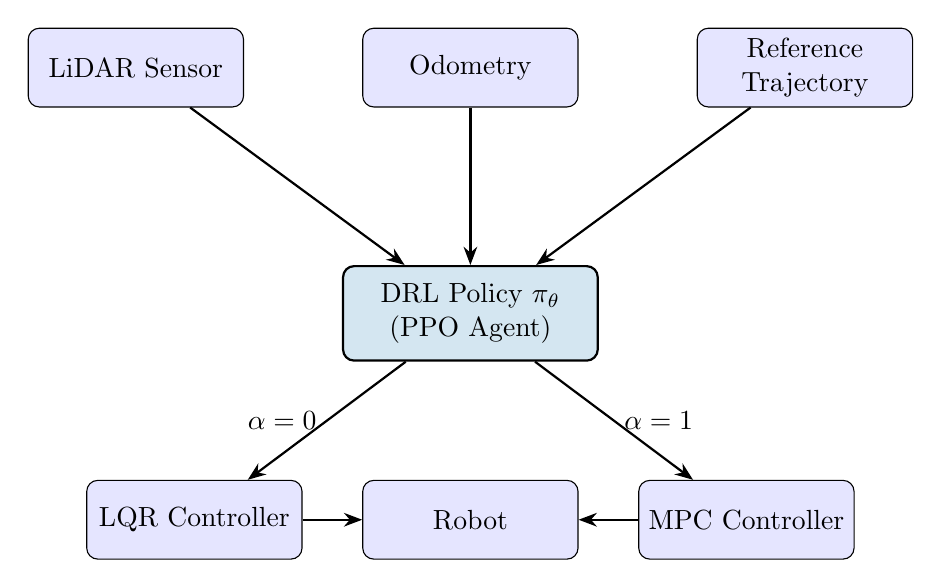
\begin{tikzpicture}[
  node distance=1.5cm,
  block/.style={rectangle, draw, fill=blue!10, text width=2.5cm, text centered, minimum height=1cm, rounded corners},
  agent/.style={rectangle, draw, fill=drlcolor!20, text width=3cm, text centered, minimum height=1.2cm, rounded corners, thick},
  arrow/.style={-Stealth, thick}
]
  % Nodes
  \node[block] (lidar) {LiDAR Sensor};
  \node[block, right=of lidar] (odom) {Odometry};
  \node[block, right=of odom] (ref) {Reference Trajectory};
  
  \node[agent, below=2cm of odom] (drl) {DRL Policy $\pi_\theta$\\(PPO Agent)};
  
  \node[block, below left=1.5cm and 0.5cm of drl] (lqr) {LQR Controller};
  \node[block, below right=1.5cm and 0.5cm of drl] (mpc) {MPC Controller};
  
  \node[block, below=1.5cm of drl] (robot) {Robot};
  
  % Arrows
  \draw[arrow] (lidar) -- (drl);
  \draw[arrow] (odom) -- (drl);
  \draw[arrow] (ref) -- (drl);
  
  \draw[arrow] (drl) -- node[left] {$\alpha=0$} (lqr);
  \draw[arrow] (drl) -- node[right] {$\alpha=1$} (mpc);
  
  \draw[arrow] (lqr) -- (robot);
  \draw[arrow] (mpc) -- (robot);
  
\end{tikzpicture}
\caption{DRL-based Switching Supervisor Architecture}
\end{figure}

\subsection{State Space Design}

\begin{equation}
  s_t = \begin{bmatrix}
    \underbrace{p_x, p_y, \theta}_{\text{Robot Pose}} \\[0.5em]
    \underbrace{e_x, e_y, e_\theta}_{\text{Tracking Error}} \\[0.5em]
    \underbrace{d_1, d_2, \ldots, d_n}_{\text{LiDAR Scans}} \\[0.5em]
    \underbrace{v_r, \omega_r}_{\text{Reference Velocity}} \\[0.5em]
    \underbrace{\kappa}_{\text{Path Curvature}}
  \end{bmatrix}
\end{equation}

\subsection{Action Space Options}

\textbf{Option A: Discrete Switching}
\begin{equation}
  a \in \{0, 1\} \quad \text{(LQR or MPC)}
\end{equation}

\textbf{Option B: Continuous Blending}
\begin{equation}
  u = \alpha \cdot u_{\text{MPC}} + (1 - \alpha) \cdot u_{\text{LQR}}, \quad \alpha \in [0, 1]
\end{equation}

\textbf{Option C: Hierarchical Control}
\begin{equation}
  a = (\text{mode}, \Delta Q, \Delta R, \Delta N)
\end{equation}
where the agent also adjusts controller parameters.

\subsection{Reward Function Design}

\begin{equation}
  R(s_t, a_t, s_{t+1}) = \underbrace{w_1 \cdot R_{\text{track}}}_{\text{Tracking}} + \underbrace{w_2 \cdot R_{\text{safe}}}_{\text{Safety}} + \underbrace{w_3 \cdot R_{\text{smooth}}}_{\text{Smoothness}} + \underbrace{w_4 \cdot R_{\text{eff}}}_{\text{Efficiency}}
\end{equation}

\textbf{Component Definitions:}

\begin{align}
  R_{\text{track}} &= -\|x - x_{\text{ref}}\|_Q^2 \\
  R_{\text{safe}} &= 
  \begin{cases}
    -100 & \text{if collision} \\
    -\frac{1}{d_{\min}} & \text{if } d_{\min} < d_{\text{warn}} \\
    0 & \text{otherwise}
  \end{cases} \\
  R_{\text{smooth}} &= -\|\Delta u\|^2 \\
  R_{\text{eff}} &= -c_{\text{switch}} \cdot \mathbf{1}[\text{mode changed}]
\end{align}

\section{DRL Implementation Roadmap}

\subsection{Training Pipeline}

\begin{algorithm}[H]
\caption{DRL Training for Switching Supervisor}
\begin{algorithmic}[1]
\State Initialize policy $\pi_\theta$ and value network $V_\phi$
\State Initialize replay buffer $\mathcal{D}$
\For{episode $= 1, 2, \ldots, N_{\text{episodes}}$}
  \State Sample environment parameters $\xi \sim p(\xi)$ \Comment{Domain randomization}
  \State Reset environment with $\xi$
  \For{$t = 0, 1, \ldots, T$}
    \State Observe state $s_t$
    \State Sample action $a_t \sim \pi_\theta(\cdot | s_t)$
    \State Execute controller based on $a_t$
    \State Observe reward $r_t$, next state $s_{t+1}$
    \State Store $(s_t, a_t, r_t, s_{t+1})$ in $\mathcal{D}$
  \EndFor
  \If{len($\mathcal{D}$) $\geq$ batch\_size}
    \State Compute advantages $\hat{A}_t$ using GAE
    \State Update $\theta$ using PPO objective
    \State Update $\phi$ using value loss
  \EndIf
\EndFor
\end{algorithmic}
\end{algorithm}

\subsection{Simulation Environment}

\begin{table}[h]
\centering
\caption{Gazebo Training Scenarios}
\begin{tabular}{lll}
\toprule
\textbf{Scenario} & \textbf{Description} & \textbf{Difficulty} \\
\midrule
Empty World & No obstacles & Baseline \\
Static Obstacles & Fixed obstacle field & Easy \\
Dynamic Obstacles & Moving obstacles & Medium \\
Narrow Passages & Tight corridors & Hard \\
Adversarial & Worst-case perturbations & Expert \\
\bottomrule
\end{tabular}
\end{table}

\section{DRL: Pros and Cons}

\begin{drlbox}[Advantages]
\begin{enumerate}
  \item \textbf{Proven Track Record}: Level 5 maturity in quadruped locomotion (ANYbotics, Boston Dynamics)
  \item \textbf{End-to-End Learning}: No need for manual feature engineering
  \item \textbf{Robustness via Domain Randomization}: Handles unseen disturbances
  \item \textbf{Publication Precedent}: Strong alignment with T-RO publication trends
  \item \textbf{Available Infrastructure}: Stable-Baselines3, Isaac Gym, ROS2 integration
\end{enumerate}
\end{drlbox}

\begin{warningbox}[Challenges]
\begin{enumerate}
  \item \textbf{Sim-to-Real Gap}: Requires extensive domain randomization
  \item \textbf{Sample Inefficiency}: Millions of samples for training
  \item \textbf{Black-Box Nature}: Difficult to interpret switching decisions
  \item \textbf{Safety During Training}: Cannot train directly on real robot
  \item \textbf{Hyperparameter Sensitivity}: Requires careful tuning
\end{enumerate}
\end{warningbox}

% ============================================================
% PART III: PATHWAY II - CAUSAL REINFORCEMENT LEARNING
% ============================================================
\newpage
\part*{\textcolor{crlcolor}{Pathway II: Causal Reinforcement Learning}}
\addcontentsline{toc}{part}{Pathway II: Causal Reinforcement Learning}

\section{Causal Reinforcement Learning: Foundations}

\subsection{What is Causal Reinforcement Learning?}

Causal Reinforcement Learning (CRL) integrates causal inference principles into RL to enable agents to understand \textit{why} certain actions lead to outcomes, not just \textit{what} outcomes occur.

\begin{crlbox}[Core Concept]
CRL learns a Structural Causal Model (SCM) of the environment, enabling counterfactual reasoning: ``What would have happened if I had taken a different action?''
\end{crlbox}

\subsection{Structural Causal Models (SCM)}

An SCM $\mathcal{M} = (\mathcal{U}, \mathcal{V}, \mathcal{F}, P(\mathcal{U}))$ consists of:
\begin{itemize}
  \item $\mathcal{U}$: Exogenous (unobserved) variables
  \item $\mathcal{V}$: Endogenous (observed) variables
  \item $\mathcal{F}$: Structural equations $V_i = f_i(\text{Pa}(V_i), U_i)$
  \item $P(\mathcal{U})$: Distribution over exogenous variables
\end{itemize}

\subsubsection{Pearl's Causal Hierarchy}

\begin{enumerate}
  \item \textbf{Association} (Seeing): $P(Y|X)$ -- observational
  \item \textbf{Intervention} (Doing): $P(Y|do(X))$ -- causal effect
  \item \textbf{Counterfactual} (Imagining): $P(Y_{X=x'}|X=x, Y=y)$ -- what-if
\end{enumerate}

\subsection{Mathematical Framework}

\subsubsection{Causal MDP (CMDP)}

A Causal MDP extends standard MDPs with causal structure:
\begin{equation}
  \mathcal{M}_C = (\mathcal{G}, \mathcal{S}, \mathcal{A}, P, R, \gamma)
\end{equation}

where $\mathcal{G}$ is a causal graph over state variables.

\subsubsection{Interventional Distributions}

The effect of action $a$ on state transition is modeled as an intervention:
\begin{equation}
  P(s'|do(a), s) = \prod_{i} P(S'_i | \text{Pa}_\mathcal{G}(S'_i), a)
\end{equation}

\subsubsection{Causal Effect Estimation}

Using the adjustment formula (back-door criterion):
\begin{equation}
  P(Y|do(X)) = \sum_Z P(Y|X, Z) P(Z)
\end{equation}

where $Z$ is a sufficient adjustment set.

\subsubsection{Counterfactual Reasoning}

For a factual observation $(x, y)$, the counterfactual under intervention $X \leftarrow x'$:
\begin{equation}
  Y_{X \leftarrow x'} = f_Y(\text{Pa}(Y), U_Y) \quad \text{with } U_Y \text{ inferred from } (x, y)
\end{equation}

\subsection{Causal Discovery Algorithms}

\subsubsection{NOTEARS (Non-combinatorial Optimization)}

Learns DAG structure by solving:
\begin{equation}
  \min_W \frac{1}{2n} \|X - XW\|_F^2 + \lambda \|W\|_1 \quad \text{s.t.} \quad h(W) = 0
\end{equation}

where the acyclicity constraint is:
\begin{equation}
  h(W) = \text{tr}(e^{W \circ W}) - d = 0
\end{equation}

\subsubsection{PC Algorithm}

Constraint-based discovery using conditional independence tests:
\begin{enumerate}
  \item Start with complete undirected graph
  \item Remove edges where $X \perp\!\!\!\perp Y | Z$
  \item Orient edges using v-structures and Meek rules
\end{enumerate}

\subsection{Causal RL Algorithms}

\subsubsection{CausalPPO}

Modifies PPO to use only causal features:
\begin{equation}
  \pi_\theta(a|s_{\text{core}}) \quad \text{where } s_{\text{core}} \subset s
\end{equation}

Only causally relevant state dimensions are fed to the policy.

\subsubsection{Counterfactual Advantage Estimation (CAE)}

\begin{equation}
  A^{\text{CF}}(s, a) = Q(s, a) - \E_{a' \sim \pi}[Q(s, a')|U]
\end{equation}

where $U$ is inferred from trajectory history.

\subsubsection{Proxy-Adjusted Causal Estimation (PACE)}

For offline learning with confounders:
\begin{equation}
  \pi^*(a|s, Z) = \argmax_\pi \E_{Z}[R(s, a, Z)]
\end{equation}

where $Z$ is a proxy variable for unobserved confounders.

\section{CRL Integration Architecture}

\subsection{Proposed Integration: Causal Risk Supervisor}

\begin{figure}[h]
\centering
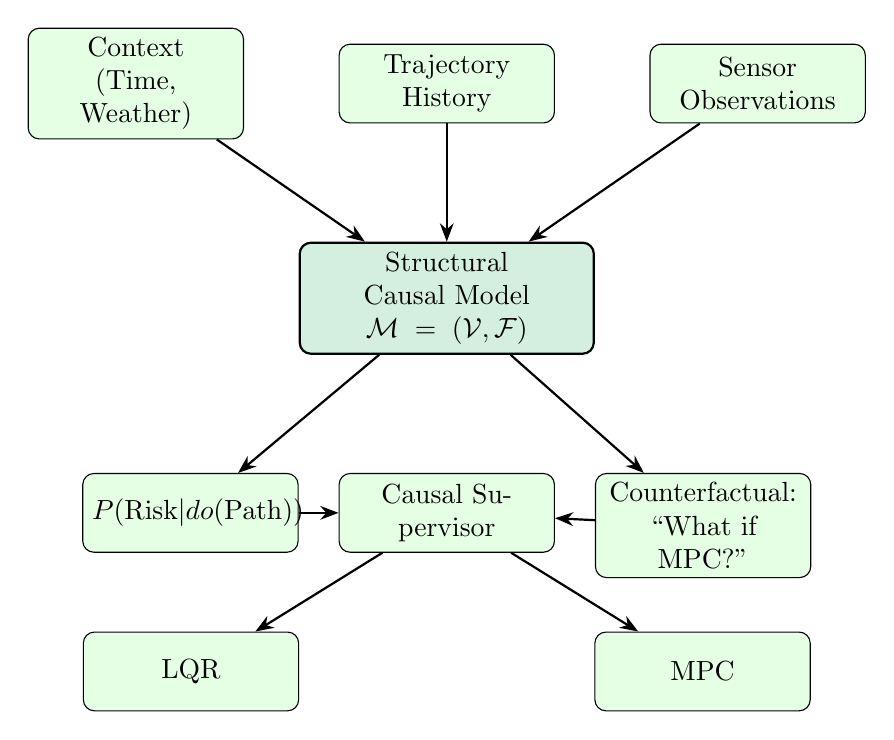
\begin{tikzpicture}[
  node distance=1.2cm,
  block/.style={rectangle, draw, fill=green!10, text width=2.5cm, text centered, minimum height=1cm, rounded corners},
  scm/.style={rectangle, draw, fill=crlcolor!20, text width=3.5cm, text centered, minimum height=1.2cm, rounded corners, thick},
  arrow/.style={-Stealth, thick}
]
  % Causal Variables
  \node[block] (context) {Context\\(Time, Weather)};
  \node[block, right=of context] (history) {Trajectory\\History};
  \node[block, right=of history] (sensor) {Sensor\\Observations};
  
  % SCM
  \node[scm, below=1.5cm of history] (scm) {Structural Causal Model\\$\mathcal{M} = (\mathcal{V}, \mathcal{F})$};
  
  % Causal Queries
  \node[block, below left=1.5cm and 0cm of scm] (risk) {$P(\text{Risk}|do(\text{Path}))$};
  \node[block, below right=1.5cm and 0cm of scm] (cf) {Counterfactual:\\``What if MPC?''};
  
  % Supervisor
  \node[block, below=1.5cm of scm] (super) {Causal Supervisor};
  
  % Controllers
  \node[block, below left=1cm and 0.5cm of super] (lqr) {LQR};
  \node[block, below right=1cm and 0.5cm of super] (mpc) {MPC};
  
  % Arrows
  \draw[arrow] (context) -- (scm);
  \draw[arrow] (history) -- (scm);
  \draw[arrow] (sensor) -- (scm);
  
  \draw[arrow] (scm) -- (risk);
  \draw[arrow] (scm) -- (cf);
  
  \draw[arrow] (risk) -- (super);
  \draw[arrow] (cf) -- (super);
  
  \draw[arrow] (super) -- (lqr);
  \draw[arrow] (super) -- (mpc);
  
\end{tikzpicture}
\caption{CRL-based Causal Risk Supervisor Architecture}
\end{figure}

\subsection{Causal Graph for Navigation}

\begin{figure}[h]
\centering
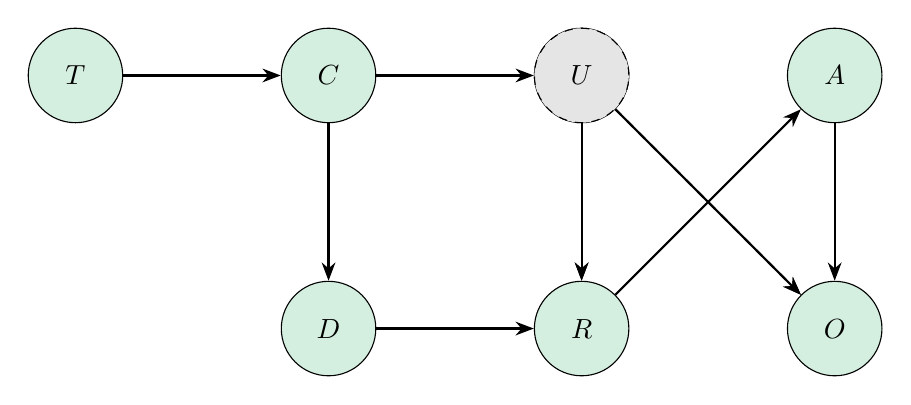
\begin{tikzpicture}[
  node distance=2cm,
  var/.style={circle, draw, fill=crlcolor!20, minimum size=1.2cm},
  hidden/.style={circle, draw, dashed, fill=gray!20, minimum size=1.2cm},
  arrow/.style={-Stealth, thick}
]
  % Variables
  \node[var] (time) {$T$};
  \node[var, right=of time] (context) {$C$};
  \node[var, below=of context] (crowd) {$D$};
  \node[var, right=of context] (sensor) {$S$};
  \node[var, below=of sensor] (risk) {$R$};
  \node[var, right=of sensor] (action) {$A$};
  \node[var, below=of action] (outcome) {$O$};
  \node[hidden, above=of risk] (U) {$U$};
  
  % Edges
  \draw[arrow] (time) -- (context);
  \draw[arrow] (context) -- (crowd);
  \draw[arrow] (context) -- (sensor);
  \draw[arrow] (crowd) -- (risk);
  \draw[arrow] (sensor) -- (risk);
  \draw[arrow] (risk) -- (action);
  \draw[arrow] (action) -- (outcome);
  \draw[arrow] (sensor) -- (outcome);
  \draw[arrow, dashed] (U) -- (risk);
  \draw[arrow, dashed] (U) -- (outcome);
  
\end{tikzpicture}
\caption{Causal DAG: $T$=Time, $C$=Context, $D$=Crowd Density, $S$=Sensor, $R$=Risk, $A$=Action, $O$=Outcome, $U$=Unobserved Confounder}
\end{figure}

\subsection{Causal Risk Estimation}

\subsubsection{Interventional Risk Query}

\begin{equation}
  P(\text{Collision}|do(\text{Mode}=\text{LQR}), \text{Context}) = \sum_S P(\text{Collision}|S, \text{LQR}) P(S|\text{Context})
\end{equation}

\subsubsection{Counterfactual Mode Selection}

Given current observation, compute counterfactual outcome:
\begin{equation}
  \text{Mode}^* = \argmin_m P(O_{\text{bad}} | \text{Mode} \leftarrow m, \text{observed trajectory})
\end{equation}

\subsubsection{Context-Aware Switching}

\begin{equation}
  P(\text{Risk}) = P(\text{Obstacle}|\text{Time}, \text{Location}, \text{Weather})
\end{equation}

Example learned relations:
\begin{itemize}
  \item Lunchtime $\rightarrow$ Canteen crowded $\rightarrow$ Higher obstacle risk
  \item Rain $\rightarrow$ Slippery floor $\rightarrow$ Longer stopping distance
  \item Night $\rightarrow$ Limited visibility $\rightarrow$ Conservative MPC
\end{itemize}

\section{CRL Implementation Roadmap}

\subsection{Causal Discovery Pipeline}

\begin{algorithm}[H]
\caption{Causal Discovery for Navigation SCM}
\begin{algorithmic}[1]
\State Collect observational data $\mathcal{D} = \{(s_t, a_t, r_t, c_t)\}_{t=1}^N$
\State Define variable set $\mathcal{V} = \{\text{Time, Location, Crowd, Sensor, Risk, Action, Outcome}\}$
\State Apply NOTEARS to learn adjacency matrix $W$
\State Prune edges using significance tests
\State Validate structure using held-out interventions
\State Return causal graph $\mathcal{G}$
\end{algorithmic}
\end{algorithm}

\subsection{SCM Training}

\begin{equation}
  \mathcal{L}_{\text{SCM}} = \sum_i \mathcal{L}_{\text{pred}}(V_i, \hat{f}_i(\text{Pa}(V_i))) + \lambda \cdot h(W)
\end{equation}

where $\hat{f}_i$ are neural network structural equations.

\section{CRL: Pros and Cons}

\begin{crlbox}[Advantages]
\begin{enumerate}
  \item \textbf{Superior Generalization}: 99.8\% gap reduction under distribution shift
  \item \textbf{Sample Efficiency}: 24.5\% faster learning (D'Cruz 2024)
  \item \textbf{Interpretability}: Explains \textit{why} decisions are made
  \item \textbf{Counterfactual Reasoning}: Can predict outcomes of untried actions
  \item \textbf{Safety}: Principled handling of confounders
  \item \textbf{High Novelty}: No prior LQR/MPC + CRL integration exists
\end{enumerate}
\end{crlbox}

\begin{warningbox}[Challenges]
\begin{enumerate}
  \item \textbf{Computational Overhead}: Causal inference adds latency
  \item \textbf{Causal Discovery Difficulty}: Identifying correct structure is hard
  \item \textbf{Limited Robotics Precedent}: Fewer established baselines
  \item \textbf{Real-Time Constraints}: May conflict with 100 Hz control loops
  \item \textbf{Higher Burden of Proof}: Reviewers may require extensive validation
\end{enumerate}
\end{warningbox}

% ============================================================
% PART IV: COMPARATIVE ANALYSIS
% ============================================================
\newpage
\part*{Comparative Analysis}
\addcontentsline{toc}{part}{Comparative Analysis}

\section{Side-by-Side Comparison}

\begin{table}[h]
\centering
\caption{DRL vs CRL Comparison for LQR/MPC Integration}
\footnotesize
\begin{tabular}{p{3cm}p{5cm}p{5cm}}
\toprule
\textbf{Aspect} & \textbf{DRL (Pathway I)} & \textbf{CRL (Pathway II)} \\
\midrule
\textbf{Novelty} & Lower (well-established) & Higher (emerging field) \\
\textbf{Publication Risk} & Lower & Higher (but recent successes) \\
\textbf{Generalization} & Brittle under domain shift & Provably robust via invariances \\
\textbf{Sample Efficiency} & Data-hungry & More efficient (counterfactuals) \\
\textbf{Interpretability} & Black-box & Causal explanations \\
\textbf{Safety} & Implicit (reward shaping) & Explicit (causal reasoning) \\
\textbf{Real-Time} & Fast (feedforward NN) & Slower (inference queries) \\
\textbf{Implementation} & Mature tools available & Requires custom implementation \\
\textbf{Validation Burden} & Standard benchmarks & Must prove methodology \\
\bottomrule
\end{tabular}
\end{table}

\section{Risk-Impact Matrix}

\begin{figure}[h]
\centering
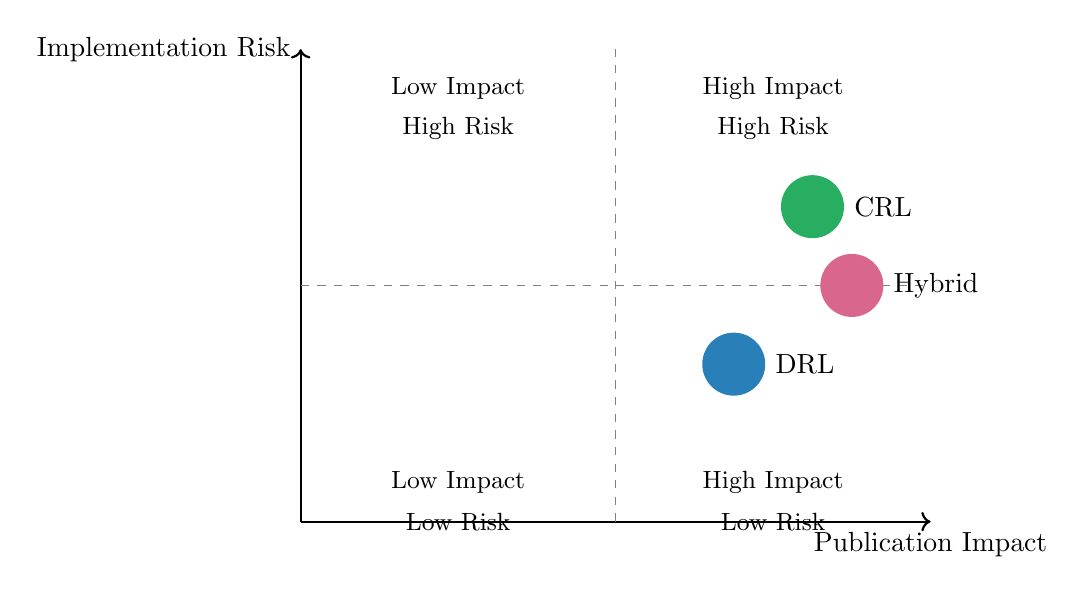
\begin{tikzpicture}
  % Axes
  \draw[thick,->] (0,0) -- (8,0) node[anchor=north] {Publication Impact};
  \draw[thick,->] (0,0) -- (0,6) node[anchor=east] {Implementation Risk};
  
  % Quadrants
  \draw[dashed, gray] (4,0) -- (4,6);
  \draw[dashed, gray] (0,3) -- (8,3);
  
  % Labels
  \node at (2,5.5) {\small Low Impact};
  \node at (2,5) {\small High Risk};
  \node at (6,5.5) {\small High Impact};
  \node at (6,5) {\small High Risk};
  \node at (2,0.5) {\small Low Impact};
  \node at (2,0) {\small Low Risk};
  \node at (6,0.5) {\small High Impact};
  \node at (6,0) {\small Low Risk};
  
  % Points
  \node[circle, fill=drlcolor, minimum size=0.8cm, label=right:DRL] at (5.5,2) {};
  \node[circle, fill=crlcolor, minimum size=0.8cm, label=right:CRL] at (6.5,4) {};
  \node[circle, fill=purple!60, minimum size=0.8cm, label=right:Hybrid] at (7,3) {};
  
\end{tikzpicture}
\caption{Risk-Impact Assessment}
\end{figure}

% ============================================================
% PART V: MVP AND X-FACTOR
% ============================================================
\newpage
\section{Minimum Viable Product (MVP)}

\subsection{DRL MVP}

\begin{enumerate}
  \item \textbf{Week 1-2}: Set up Gazebo simulation with domain randomization
  \item \textbf{Week 3-4}: Implement PPO agent using Stable-Baselines3
  \item \textbf{Week 5-6}: Train switching supervisor (discrete action)
  \item \textbf{Week 7-8}: Evaluate on test scenarios, tune hyperparameters
\end{enumerate}

\textbf{Deliverable}: Trained DRL policy that switches LQR/MPC with >90\% success rate in simulation.

\subsection{CRL MVP}

\begin{enumerate}
  \item \textbf{Week 1-2}: Collect observational data from simulation
  \item \textbf{Week 3-4}: Implement NOTEARS for causal discovery
  \item \textbf{Week 5-6}: Train SCM with neural structural equations
  \item \textbf{Week 7-8}: Implement causal risk queries, integrate with supervisor
\end{enumerate}

\textbf{Deliverable}: Causal model that predicts risk and explains switching decisions.

\section{X-Factor: Differentiating Contribution}

\subsection{DRL X-Factor}

\begin{drlbox}[Unique Contribution]
\textbf{Adaptive Parameter Tuning}: The DRL agent not only selects the controller mode but also adjusts controller parameters $(Q, R, N)$ in real-time based on environmental conditions.

\begin{equation}
  a = (\text{mode}, \Delta Q, \Delta R, \Delta N_{\text{horizon}})
\end{equation}

This creates a \textbf{meta-controller} that optimizes the optimization.
\end{drlbox}

\subsection{CRL X-Factor}

\begin{crlbox}[Unique Contribution]
\textbf{Anticipatory Mode Switching}: The causal model predicts obstacles \textit{before} they are detected by LiDAR, using contextual cues:

\begin{equation}
  P(\text{Obstacle}_{t+\Delta t} | \text{Context}_t) > \tau \implies \text{Preemptive MPC}
\end{equation}

This is the \textbf{first integration of causal reasoning with LQR/MPC switching}.
\end{crlbox}

\subsection{Hybrid X-Factor}

\begin{warningbox}[Maximum Impact Strategy]
\textbf{Combine Both}: Use CRL for high-level anticipatory decisions and DRL for low-level adaptive control:

\begin{enumerate}
  \item CRL predicts risk horizon and triggers MPC preemptively
  \item DRL fine-tunes controller parameters based on immediate feedback
  \item Causal model provides interpretable explanations
  \item DRL provides robust handling of edge cases
\end{enumerate}
\end{warningbox}

% ============================================================
% PART VI: REAL-WORLD IMPLICATIONS
% ============================================================
\section{Real-World Implications and Applications}

\subsection{Application Domains}

\begin{table}[h]
\centering
\caption{Target Application Scenarios}
\begin{tabular}{lll}
\toprule
\textbf{Domain} & \textbf{DRL Benefit} & \textbf{CRL Benefit} \\
\midrule
Warehouse Robots & Robust locomotion & Crowd prediction \\
Autonomous Vehicles & Agile maneuvering & Safety guarantees \\
Hospital Robots & Dynamic obstacle handling & Explainable decisions \\
Agricultural Robots & Terrain adaptation & Weather reasoning \\
\bottomrule
\end{tabular}
\end{table}

\subsection{Deployment Considerations}

\begin{itemize}
  \item \textbf{Computational Requirements}: DRL requires GPU for training; CRL requires efficient inference
  \item \textbf{Certification}: CRL's interpretability aids regulatory approval
  \item \textbf{Maintenance}: CRL models may need updating as environment changes
  \item \textbf{Fallback}: Both require safe fallback to pure LQR/MPC
\end{itemize}

% ============================================================
% PART VII: RECOMMENDATION
% ============================================================
\section{Strategic Recommendation}

Based on this analysis, we recommend a \textbf{phased approach}:

\subsection{Phase 3A: DRL Integration (Months 1-3)}

\begin{enumerate}
  \item Implement PPO-based switching supervisor
  \item Achieve robust sim-to-real transfer
  \item Establish baseline performance metrics
\end{enumerate}

\subsection{Phase 3B: CRL Enhancement (Months 4-6)}

\begin{enumerate}
  \item Add causal risk prediction layer
  \item Implement anticipatory switching
  \item Generate interpretable explanations
\end{enumerate}

\subsection{Publication Strategy}

\begin{enumerate}
  \item \textbf{Conference Paper} (ICRA/IROS): DRL-enhanced hybrid controller
  \item \textbf{Journal Paper} (T-RO/RAL): Full CRL+DRL framework with theoretical analysis
  \item \textbf{Workshop Paper}: Interpretability and safety analysis
\end{enumerate}

% ============================================================
% CONCLUSION
% ============================================================
\section{Conclusion}

This proposal has presented two complementary pathways for enhancing our Risk-Aware Hybrid LQR-MPC Navigation system. Deep Reinforcement Learning offers a proven, mature approach with strong publication precedent, while Causal Reinforcement Learning offers higher novelty and addresses fundamental limitations of standard RL. 

The optimal strategy combines both: using CRL for anticipatory, interpretable high-level decisions and DRL for robust, adaptive low-level control. This hybrid approach maximizes both the technical contribution and the publication impact.

% ============================================================
% REFERENCES
% ============================================================
\newpage
\bibliographystyle{plain}
\begin{thebibliography}{99}

\bibitem{schulman2017ppo} Schulman, J., et al. ``Proximal Policy Optimization Algorithms.'' arXiv:1707.06347, 2017.

\bibitem{castri2026} Castri, L., et al. ``Causality-enhanced Decision-Making for Autonomous Mobile Robots in Dynamic Environments.'' arXiv:2504.11901, 2026.

\bibitem{dcruz2024} D'Cruz, N., et al. ``Causal Reinforcement Learning for Optimisation of Robot Dynamics in Unknown Environments.'' arXiv:2409.13423, 2024.

\bibitem{tang2024} Tang, X., et al. ``Causal Deconfounding Deep Reinforcement Learning for Mobile Robot Motion Planning.'' Knowledge-Based Systems, 2024.

\bibitem{lin2024} Lin, H., et al. ``Safety-aware Causal Representation for Trustworthy Offline Reinforcement Learning in Autonomous Driving.'' arXiv:2311.10747, 2024.

\bibitem{wu2025} Wu, Z., et al. ``Causal Correction and Compensation Network for Robotics: Applications and Validation in Continuous Control.'' Applied Sciences, 2025.

\bibitem{pearl2009} Pearl, J. ``Causality: Models, Reasoning, and Inference.'' Cambridge University Press, 2009.

\bibitem{zheng2018notears} Zheng, X., et al. ``DAGs with NO TEARS: Continuous Optimization for Structure Learning.'' NeurIPS, 2018.

\bibitem{crlsurvey} ``Unifying Causal Reinforcement Learning: Survey, Taxonomy, Algorithms and Applications.'' arXiv:2512.18135, 2024.

\end{thebibliography}

\end{document}
